\chapter{Residential Location Choice}
\section{Introduction}
Dual-worker households are an increasingly important subset of household arrangements in the analysis of transportation behaviour. Increasing costs of living relative to wages necessitate additional sources of income for the household. The proportion of dual-worker households in Canada rose from 38\% in 1976 to 70\% in 2015 \cite{StatisticsCanada2017}. In the context of transportation behaviour, dual-worker households negotiate over limited resources (e.g. the number of household vehicles or mobility tools) to minimize their journey-to-work travel expenditure (time and costs). Capturing such interactions of household members and their inclination towards compromise or shared travel are critical in modelling residential location choices of dual-worker households. Conventional univariate decision theories are insufficient to model such choice contexts. Ho and Mulley \cite{Ho2015,Ho2015a}, as well as Akbari and Habib \cite{Akbari2015}, suggest that short and long-term decisions (e.g. home location, auto ownership, and proximity to rail transit choices) that are conventionally modelled at the level of the household are in fact composite decisions resulting from trade-offs between members (joint decisions) of the household to achieve a reasonable level of household utility. However, applications of household level composite utility-based joint decision theory in transport modelling have been scarce and it is a pressing issue in household-based travel demand investigation \cite{Picard2013}. The present research contributes to this critical research gap by presenting a Random Utility Maximization (RUM) based joint decision model of home location choice, considering multiple worker households. Residential location choice is considered from the perspective of bid-rent, locations choosing households with the highest bids, and utilize the latent auction approach recently proposed by Hurtubia \emph{et al.} \cite{Hurtubia2017}. The paper breaks new ground of exploiting the latent auction approach to accommodate the intra-household interactions in home location choice modelling. For empirical application, we use a combination of revealed preference (RP) and stated preference (SP) data collected in the Greater Toronto Area (GTA) and real estate statistics to estimate a model with household and individual-specific components of utility.

\section{Model Formulation}
In developing the model, we employ the bid-auction approach developed by Hurtubia \cite{Hurtubia2012}, which builds upon the bid-choice theory of Martinez. Model derivation begins with a standard bid-rent function \cite{Ellickson1981} defined as follows:
\begin{equation}
	P(h|i) =  \frac{\exp\left(\mu B_{hi} \right)}{\sum\limits_{g \in H} \exp\left(\mu B_{gi} \right)} ,
\end{equation}

where $P(h|i)$ is the probability of household $h$ being located in TAZ $i$. The bid $B_{hi}$ can be parameterized as a function of zonal and household characteristics, and the winning bid expressed as a stochastic expectation as follows:
\begin{equation}
	r_i =  E\left(max_H\left(B_{hi}\right)\right) = \frac{1}{\mu} ln\left(\sum_{g \in H} \exp\left(\mu B_{gi}\right)\right) ,
\end{equation}
which, according to bid-choice theory \cite{Martinez1992a}, gives an equivalent distribution of households to the location choice formulation of Lerman \cite{Lerman1976}. The logsum term gives a standard measure of the expected maximum bid for a particular location $i$.

Hurtubia works from this basis to develop a microsimulation of the bid-choice process \cite{Hurtubia2012}. He proposes a latent variable approach, wherein the bids of all households who consider a particular location are included in the price, but only in relative terms. To estimate this latent bid-auction, the observed price $R_i$ can be represented as a function of the latent auction price $r_i$ as follows:
% * <khandker.nurulhabib@utoronto.ca> 2018-07-06T08:24:38.693Z:
% 
% In other way, you can say that:
% It is assumed to follow a normal distribution and then show the equation
% 
% ^ <khandker.nurulhabib@utoronto.ca> 2018-07-06T08:29:26.126Z.
\begin{equation}
f(R_i|r_i) =  \frac{\exp\left(- \frac{R_i-a-\gamma r_i}{2\sigma^2}\right)}{\sqrt{2\pi\sigma^2}} ,
\end{equation}
where $\alpha$, $\gamma$, and $\sigma$ are estimated parameters representing the relationship between the observed and latent prices for location $i$. Assuming a mean of zero, the above function represents the probability of the observed price, given the latent price derived from the logsum auction price. The likelihood term is then a function of the product of the bid-rent probability and the price density function:
\begin{equation}
\mathcal{L} = P(h|i)f(R_i|r_i)
\end{equation}

We see this is an appealing framework for the development of a residential location choice model. It is consistent with the microeconomic foundations of bid-choice and provides a method for the inclusion of endogenous prices in an agent-based microsimulation model. The inclusion of intrahousehold dynamics is accomplished through a modification of the parameterized bid function $B_{hi}$. The decision of a residential location is a function of both household and individual-specific attributes, which can be considered through a weighted utility function. The bid function is then given by:
\begin{equation}
B_{hi} =  \sum_j \beta_j X_{hj} + \sum_k \beta_k Z_{hik} + \sum_{p \in h} \left(w_p \sum_m \beta_m X_{hm} + \sum_n \beta_n Z_{hin}\right) ,
\end{equation}
where $X_{hj}$ are household-specific explanatory variables, $Z_{hik}$ are terms that interact household and location-specific explanatory variables, $X_{hm}$ are individual-specific explanatory variables, and $Z_{hin}$ are terms that interact individual and location-specific explanatory variables. The individual-specific weights can be parameterized as logit functions of sociodemographic characteristics as follows:
\begin{equation}
w_p = \frac{\exp \left( \sum_s \alpha_s y_{ps} \right)}{\sum\limits_{p \in h} \exp \left( \sum_s \alpha_s y_{ps} \right)} ,
\end{equation}
where $y_{ps}$ are individual-specific sociodemographic variables describing the weight of the utility associated with individual $p$ of household $h$.
\section{Data Description}
The empirical application is based on a survey conducted in 2014 by residents of the GTA. The survey, denoted CHOICE for \underline{C}ar and \underline{H}ousehold \underline{O}wnership in the face of \underline{I}ncreasing \underline{C}ommuting \underline{E}xpenses, focuses on car and home ownership decisions \cite{Papaioannou2014}. It includes a large set of RP data regarding car and home characteristics, as well as sociodemographic information on each responding household. Two stated preference (SP) experiments are included in the survey, focusing on mobility tool adoption and residential location choice, respectively. A total of 501 complete responses were acquired through a panel provided by the market research firm Research Now \cite{Papaioannou2014}. From this sample, 413 household responses - including information on 757 individuals - are used in the present analysis. The CHOICE survey data are linked with additional statistics from the 2006 Transportation Tomorrow Survey (TTS) to calculate interzonal travel times and costs, which we update with data from the 2011 survey \cite{Papaioannou2014,DataManagementGroup2014}. The original survey application was to interregional commuting trips. As such, the data do not include households who commute within their city of residence. This biases the average trip length of the sample, but should not adversely affect the analysis of intrahousehold dynamics. A summary of key transportation statistics is provided by household in Table ~\ref{tab:data_sum} for each of the five regions included in the analysis.

\begin{table}[H]
\caption{Descriptive statistics for key HH transportation variables.}
  \label{tab:data_sum}
  \centering
\begin{tabular}{l l c c c c c c}
  \toprule
Variable & Statistic & Durham & Halton & Peel & Toronto & York & Total \\
\midrule
\makecell[l]{Transit pass\\(0/1)} & \makecell[l]{Count of\\respondents} & 10 & 9 & 12 & 4 & 5 & 41 \\
 & \makecell[l]{Percent of\\respondents} & 8.0 & 12.9 & 11.4 & 3.3 & 10.6 & 8.6 \\
\makecell[l]{Auto + transit\\cost (monthly)} & Mean & 702 & 669 & 619 & 500 & 723 & 630 \\
\makecell[l]{Household\\vehicles} & Mean & 1.9 & 2.2 & 1.9 & 1.4 & 2.1 & 1.8 \\
\makecell[l]{Auto commuting\\time (min.)} & \makecell[l]{Mean for\\adult male} & 21.8 & 50.2 & 32.0 & 28.6 & 48.1 & 31.8 \\
& \makecell[l]{Mean for\\adult female} & 19.6 & 41.7 & 28.3 & 27.5 & 41.4 & 28.7 \\
& \makecell[l]{Mean for\\dependent child} & 18.5 & 38.4 & 28.4 & 33.8 & 45.9 & 29.4 \\
& \makecell[l]{Mean for other\\member} & 8.3 & 32.8 & 69.0 & 38.8 & & 30.9 \\
\bottomrule
\end{tabular}
\end{table}

Additional data pertaining to land use were available from regional transportation models and previous data collection by the University of Toronto. Figure ~\ref{fig:area_use} shows the distribution of land uses by classification for each of the five regions. It is clear that parks and open space still dominate the region, but residential uses are not far behind (if not higher). 

\begin{figure}[H]
\centering
        \begin{tikzpicture}
        \node[inner sep=0pt] (A) {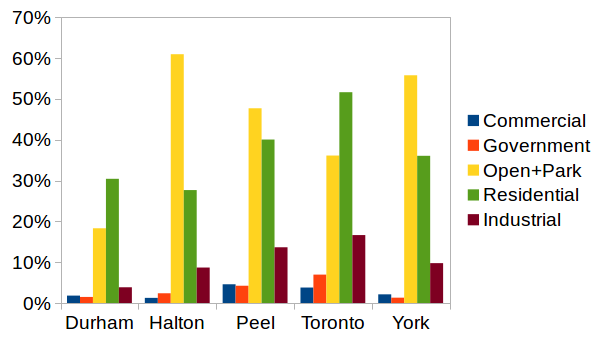
\includegraphics[width=0.7\textwidth]{media/area_use.png}};
%        \node[black] (B) at ($(A.south)!-.03!(A.north)$) {Region};
        \node[black,rotate=90] (C) at ($(A.west)!-.03!(A.east)$) {Percent of total land};
      \end{tikzpicture}
\caption{\label{fig:area_use}Distribution of region land uses.}
\end{figure}

The CHOICE survey includes data on home purchase price, or rent, but this does not give a clear picture of the overall market conditions and prices are given as of the year of purchase \cite{Papaioannou2014}. We supplement the survey data with real estate statistics compiled by the Toronto Real estate Board (TREB) \cite{TorontoRealEstateBoard2017}. They publish a monthly report outlining market prices aggregated to a custom set of 30 zones outside the City of Toronto and 36 zones within it. The TREB report classifies dwellings as detached, semi-detached, row/townhouse, condo townhouse, condo apartment, cooperative apartment, detached condo, and co-ownership apartment. We aggregate these classifications into house, townhouse, and condo for ease of analysis and to increase the sample size of each category. We further supplement these data with multiple listings service (MLS) records collected in May 2017 for both owned and rented dwellings. These data also include the area of each dwelling, number of bedrooms, and number of bathrooms. Figure ~\ref{fig:real_estate_price} provides annualized costs for each region and tenure type. For owned dwellings, a 25-year amortization period is employed, with an interest rate of 5\%, to obtain a representative annual cost \cite{RBC2018}. In the figure, each of the numbers (1,2,3) corresponds to a dwelling type (respectively: house, townhouse, and condo). It is evident that owned prices are significantly higher than rented prices; however, ownership gives the household possession of the asset and therefore includes an expected monetary return upon sale of the asset.

\begin{figure}[H]
\centering
        \begin{tikzpicture}
        \node[inner sep=0pt] (A) {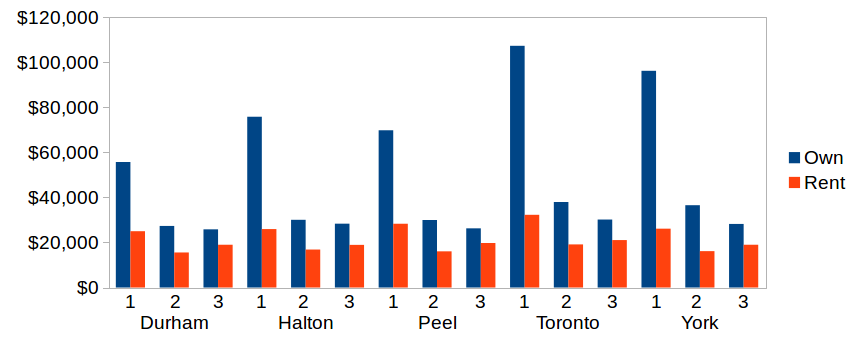
\includegraphics[width=\textwidth]{media/real_estate_price.png}};
%        \node[black] (B) at ($(A.south)!-.03!(A.north)$) {Region and Dwelling Type};
        \node[black,rotate=90] (C) at ($(A.west)!-.03!(A.east)$) {Annualized cost (\$)};
      \end{tikzpicture}
\caption{\label{fig:real_estate_price}Distribution of annualized cost by region and dwelling type.}
\end{figure}

\section{Model development}
The estimation of the bid-rent model requires multiple household agents to bid on each TAZ, with the winning agent being the one that is located in that TAZ. Using the RP data collected in the CHOICE survey, we only have the chosen location of each responding household and their characteristics. McFadden has proven that consistent parameter estimation can be performed using a random sample of alternative agents. Many previous studies of residential location choice use a smaller sample, but Nerella and Bhat provide a quantification of the error associated with smaller sampling rates \cite{Nerella2004}. Guided by their analysis, we take the household records from the CHOICE survey and associate them with 30 randomly selected households records from among those respondents who are not located in the same TAZ. We also explored a stratified importance sampling, taking 15 records from the same region and 15 from the same income group. However, this did not improve the significance of parameters or model goodness-of-fit. We define separate zones for each of the dwelling types considered in the model (i.e. house, townhouse, and condo), representing a simultaneous choice of zone and dwelling type by each household.

In most instances, unique explanatory variables can only be derived from the interaction of zone and household-specific attributes. A summary of the variables included in the final model is provided in Table ~\ref{tab:var_sum}. For example, the commuting drive time to work is a function of both the home and work location of a respondent. We assume that work locations are fixed, but the use of a record in the estimation of the expected bid in another TAZ requires an estimate of the commuting time from this unchosen home location. We, therefore, link the data with an inter-zonal matrix of AM peak auto commuting times from the GTA RTM. A second example of this interaction is the average dwelling area for each TAZ, which we interact with a household size of the respondent. Taking the natural logarithm of the household size provides a measure of dwelling area having a diminishing marginal influence on choice for each additional household member. In some instances, only the household attribute is used, as in the case of home to work distance. We divide this value by the income of each individual to obtain a measure of the sensitivity to commuting distance as a function of additional income. We assume this sensitivity to be a characteristic of the individual, independent of the TAZ they are considering - in contrast to the commuting time sensitivity, which is assumed fixed across respondents. The combination of these two variables accounts for the effect of proximity to the work location and differences between individuals arising from economic factors.

We define alternative-specific constants (ASC) by the membership of each household in an income quintile. This is similar to the models developed by Hurtubia in his original work \cite{Hurtubia2012}. In this initial exploration of the model, we define the individual utility weights by household role. Four roles are defined as follows: adult male, adult female, dependent child, and other member. It should be noted that there is some overlap between the characteristics of individuals holding an "adult" or "child" role in the dataset. The "child" role generally refers to individuals under the age of 18, but may include older individuals who still live with their parents (e.g. university students). This distinction is deemed valid as the weights denote the role each individual plays in determining the residential location choice. In the case of an individual, over the age of 18 and living at home, it is likely they were younger at the time of the residential location choice. In contrast, the same individual likely had a greater influence on the decision if they are listed as an "adult" and they are the owner of the dwelling. This partially explains the result in Table ~\ref{tab:data_sum}. The average commuting time for those given the role "child" is similar to, or higher than, the "adult" roles for most regions. There are two households with individuals listed as "child" who are aged 35 to 44. With the caveat that the sample size makes this largely anecdotal, the mean commuting time for these individuals is 47 minutes, which is well above the regional average.

\begin{longtable}{l r l}
\caption{Development of model variables.}
  \label{tab:var_sum}\\
  \toprule
Variable &    TAZ property $\times$ &  HH property \\
\midrule
\endfirsthead
\caption[]{(continued)}\\
\toprule
Variable &    TAZ property $\times$ &  HH property \\
\midrule
\endhead
\multicolumn{3}{c}{\textbf{Individual Variables}} \\
HW distance & & \makecell[l]{Home to work commute\\distance / individual income} \\
HW auto time & \makecell[r]{Inter-zonal home-to-work\\auto travel time (min.)} & Exogenous work TAZ \\
Park cost & & \makecell[l]{Cost of parking at work\\location (10s \$ per month)} \\
Transit & \makecell[r]{Count of GO Train stations within\\3 km or TTC stations within 500 m\\of zone centroid} & \makecell[l]{Individual has transit\\pass (0/1)} \\
\makecell[l]{Frequency\\auto} & & \makecell[l]{Frequency of individual\\commute by auto} \\
HW TAZ & \makecell[r]{Home and work location\\in same TAZ (0/1)} & Exogenous work TAZ  \\
\multicolumn{3}{c}{\textbf{Household Variables}} \\
House & House (0/1) & 2+ HH members (0/1) \\
High income & \makecell[r]{Mean HH income in top\\income quintile (0/1)} & \makecell[l]{HH income in top\\income quintile (0/1)}  \\
Low income & \makecell[r]{Mean HH income in top\\income quintile (0/1)} & \makecell[l]{HH income in bottom\\income quintile (0/1)}  \\
Dwelling area & \makecell[r]{Average dwelling\\area (100s $m^2$)} & ln(HH size)  \\
Veh/lic & & HH vehicles / HH licenses  \\
Children & & Number of children in HH  \\
INC\_2 & & HH income in 2nd quintile \\
INC\_3 & & HH income in 3rd quintile \\
INC\_4 & & HH income in 4th quintile \\
INC\_5 & & HH income in top quintile \\
\multicolumn{3}{c}{\textbf{Weights}} \\
W\_Role1 & & Adult male \\
W\_Role2 & & Adult female \\
W\_Role3 & & Dependent child \\
W\_Role4 & & Other member \\
W\_Age & & Age of HH member \\
\bottomrule
\end{longtable}

\section{Model Estimation Results}
The results of the estimation are outlined in Table ~\ref{tab:model_sum} for the final model. A wide variety of intermediate models were estimated, including standard bid-rent models (excluding the latent auction component) for each model. The majority of the parameters are significant (at the 0.05 level of significance) and have intuitive signs. Critically, home to work auto travel time has a negative parameter and dwelling area is found to have a positive parameter, both being significant. The house variable - representing the probability of a household with 2, or more, members choosing a house dwelling type - has a negative sign. Looking at the corresponding bid-rent function, the sign is consistently positive in models that include this variable. Hurtubia \emph{et al.} obtain a similar result for this variable \cite{Hurtubia2017}, which are concentrated in more outlying areas of the GTA. These outlying areas are characterized by lower dwelling prices, relative to those in the City of Toronto proper. The negative sign on the parameter suggests that larger households, who have higher living expenses, value the lower priced houses located in the outlying suburbs.

We find a common parameter value for locating proximate to TTC stations and GO Train stations, given the bounding radii defined for each station type. This suggests that households tend to \emph{ceteris paribus} value being located within 500 m of a TTC station in a similar way to being located within 3 km of a GO Train station. A negative sign is obtained for the number of vehicles per licensed driver, which suggests that households tend to trade-off a higher priced dwelling against the ownership of additional vehicles. This is consistent with other parameter values in that transit proximity is positively valued and larger households tend to locate in outlying areas, with poor transit service, requiring the purchase of additional vehicles.

With respect to individual weights, weights are estimated in the final model for four household roles (i.e. adult male, adult female, dependent child, and other). A challenge in estimating these weights is the requirement for a reference weight in the MNL weight function, against which to measure the relative utility for other household members. Household compositions in the sample are not uniform, such that a single role cannot be fixed as the reference. For example, a household may contain two adult males or no adult males. We reference the weight of each household member against the role of the responding member. It is interesting to note that this model does not suggest a strong difference in the weight of male and female influence on residential location choice - in contrast to prior studies on the subject \cite{Chiappori2014, Picard2013}. In a household with a single male/female couple, the weights are 0.49 and 0.51, respectively. Given the aforementioned caveats about the overlap between "adult" and "child" roles, we included a weighting variable for the age of the household member. Although not strongly significant, this suggests that age plays a strong role in the weight of the individual on residential location choice. We explored the inclusion of several other variables, including individual work status and income, but the sample data is incomplete for these variables and their inclusion did not have a significant effect on the model.

\begin{longtable}{lrrr}
\caption{Model parameter statistics.}
\label{tab:model_sum} \\
\toprule
Variable &    Value &  Std err. &    t-stat \\
\midrule
\endfirsthead
\caption[]{(continued)}\\
\toprule
Variable &    Value &  Std err. &    t-stat \\
\midrule
\endhead
\multicolumn{4}{c}{\textbf{Individual Variables}} \\
HW auto travel time & -0.03 & 0.003 & -11.84 \\
Parking cost at school or work & 0.02 & 0.006 & 2.45 \\
Transit & 0.35 & 0.12 & 2.99 \\
Frequency auto & 1.99 & 0.17 & 11.43 \\
HW TAZ & 0.63 & 0.10 & 6.27 \\
\multicolumn{4}{c}{\textbf{Household variables}} \\
House & -0.31 & 0.02 & -14.29 \\
High income & 0.28 & 0.10 & -3.04 \\
Low income & -0.25 & 0.21 & -1.16 \\
HW distance & 1.16 & 0.24 & 4.87 \\
Dwelling area & 0.26 & 0.04 & 6.20 \\
Veh/lic & -0.52 & 0.08 & -6.58 \\
Children & -0.15 & 0.05 & -3.01  \\
INC\_2 & 0.08 & 0.27 & 0.32 \\
INC\_3 & 0.36 & 0.19 & 1.91 \\
INC\_4 & 0.38 & 0.20 & 1.90 \\
INC\_5 & 0.37 & 0.19 & 1.96 \\
\multicolumn{4}{c}{\textbf{Weights}} \\
W\_Role1 & -0.93 & 0.53 & -2.39 \\
W\_Role2 & -0.87 & 0.64 & -2.24 \\
W\_Role3 & -1.18 & 0.64 & -3.24 \\
W\_Role4 & -0.74 & 0.46 & -2.63 \\
W\_Age & -0.12 & 0.28 & -1.10 \\
\multicolumn{4}{c}{\textbf{Price variables}} \\
$\gamma$ & 0.41 & 0.04 & 9.73 \\
$\alpha$ & 9.17 & 0.21 & 43.04 \\
$\sigma$ & 0.25 & 0.006 & 39.49 \\
$\rho^2$ (const) & 0.04 & & \\ 
$\rho^2$ (null) & 0.04 & & \\ %(Hurtubia gets just under 0.10 in thesis using larger dataset.
\bottomrule
\end{longtable}

Another avenue of exploration was considering variation in household composition by distinguishing the adult role weights based on whether the household includes children. This would account for differences in the role of an adult by their consideration for school location and altruism for their children. However, no significant difference was found between these variables. This effect is partially considered through the inclusion of the age weight and variable in the household utility function indicating whether the household includes children (under the age of 13). A series of other weight configurations were explored for adult roles including: separate weights for single and multi-worker household adults, separate weights for single and multi-member household adults, and the addition of a weight for full-time work status. We also considered models wherein the individual utilities were separated into weighted and unweighted components. None of these changes significantly improved the model fit or provided statistical insights into intra-household dynamics.

\subsection{Elasticity analysis}
A robust and tangible method of examining the magnitude of parameter values is obtained from calculation of the elasticities with respect to each explanatory variable. In the case of continuous variables, this takes the form of a point elasticity, while category variables require the use of an arc elasticity measured between variable states. We present a combined plot for a subset of continuous variables in Figure ~\ref{fig:elasticity}. It is evident that there is a large positive elasticity between the probability of a household choosing to locate in a TAZ and the average dwelling area for that TAZ-dwelling type pair. A graphical representation helps to draw out the similarity in elasticities between the adult male/female roles with respect to their sensitivity to auto travel time and parking cost at school or work. It is also clear that the influence of dependent children on residential location choice is weaker.

\begin{figure}[H]
\centering
        \begin{tikzpicture}
        \node[inner sep=0pt] (A) {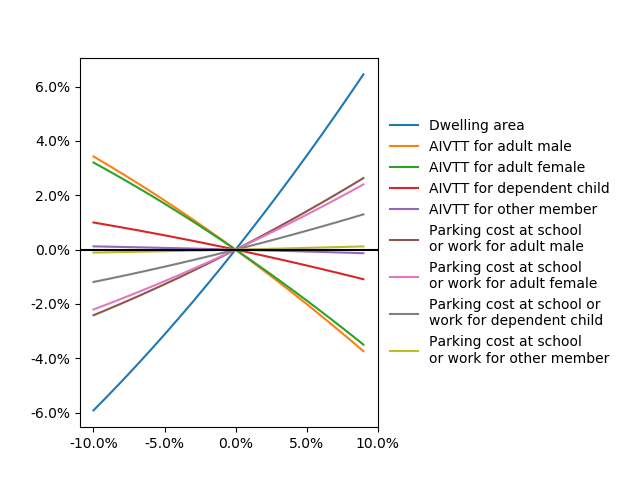
\includegraphics[width=1.0\textwidth]{media/elasticity.png}};
        \node[black] (B) at (-1.75,-5) {\% change in variable value};
        \node[black,rotate=90, align=center] (C) at ($(A.west)!-.02!(A.east)$){\% change in probability\\of HH being located in TAZ};
      \end{tikzpicture}
\caption{\label{fig:elasticity}Elasticities for representative variables.}
\end{figure}

\section{Discussion of Model Results}

\section{Chapter Conclusions}
This paper adds to the growing literature on intra-household dynamics in residential location choice. By considering such dynamics, we can better capture the decision-making process and consider a wider range of policy scenarios. We provide an independent confirmation of the bid-auction approach recently proposed by Hurtubia \emph{et al.} \cite{Hurtubia2017}. The present analysis suggests a weakening differential in the influence of male and female household members on residential location choice. This fits with a continued shift towards higher labour force engagement, whereby the household must consider the work location of several members. We find that larger households remain constrained in their ability to locate in urban areas, proximate to their work location. Whether this is an outcome of high land prices or a lack of available housing stock, single-family houses continue to be the domain of outlying suburban areas, with low land prices and high automobile dependence.

This study presents a strong basis for further research. However, it could be improved through the collection of a sample that includes households who work within the same city. A major bias, existing in most residential location choice models, is the so-called modifiable areal unit problem (MAUP). This arises from the use of arbitrary aggregations of spatial units, a standard practice in residential location choice models. We explored the inclusion of a spatial lag term in our model to account for this bias. Lags were considered for the co-location of similar income households, similar sized households, and by tenure (i.e. own or rent dwelling). Results are preliminary, but this direction holds promise for additional insights with respect to household dynamics and social factors.